\documentclass[11pt]{article}
\usepackage[margin=.75in]{geometry}
\usepackage{lmodern,amsmath,booktabs,graphicx,xcolor,pdflscape}
\usepackage[colorlinks=true,urlcolor=teal,citecolor=teal]{hyperref}
\title{When a history rule beats a pooled auction-demand model\\\large Announcement-field lineage, maturity transfer and issuance-size evidence}
\author{James Jean\\Independent research}
\date{28 October 2026\\GitHub research manuscript; not peer reviewed}
\begin{document}\maketitle
\begin{abstract}
Adding a fitted model is useful only when it improves a credible reference forecast on data outside estimation. This study compares fourteen prespecified Treasury auction-demand candidates, reconstructs every predictor's earlier-result lineage, and separates later-period evaluation from a maturity excluded from fitting and selection. The previous-six same-maturity mean has the lowest validation MSE among three historical rules, four ridge penalties, three forest depths and four boosting settings. On forty-five later ten-year auctions, its RMSE is 0.1074 bid-to-cover ratio units versus 0.1147 for the corresponding median. On 270 other-term auctions, the two are essentially tied at 0.1225 and 0.1224. Large offering-size changes are rare, limiting the proposed stress comparison. The analysis supports keeping a transparent reference forecast while a vintage-aware alternative earns added complexity. Current historical values make the experiment retrospective; it does not establish original-release performance or an investment return.
\end{abstract}
\section{The forecasting question}
An auction-research workflow may need a reference expectation for demand before the result arrives. A pooled model can use announced offering size, maturity and calendar structure, but additional parameters do not automatically produce a better forecast. A useful comparison must preserve the information boundary, retain unsuccessful candidates and show whether the selected method transfers beyond the maturities used in estimation.

The relationship between offering size and bid-to-cover ratios is already studied. GAO's 2026 debt-management report uses maturity and fiscal-year fixed effects and explicitly limits causal and out-of-sample interpretations \cite{gao}. This experiment addresses a narrower predictive implementation: earlier-auction lineage, a later evaluation period and a maturity excluded from parameter estimation. It does not introduce a new algorithm or establish an exhaustive research gap. The practical contribution is an auditable decision about whether the tested fitted models earn replacement of a simple historical reference.
\section{Official source and accounting}
The Bureau of the Fiscal Service's Treasury Securities Auctions Data API supplies 6,046 records with auction dates from 1 January 2009 through 30 September 2026 \cite{treasury}. The bounded retrieval uses seven pages and retains exact queries, field metadata, response hashes and retrieval time. Strings indicating missing values are treated as missing, never zero. The analysis keeps nominal fixed-rate notes and bonds with original terms of two, three, five, seven, ten, twenty or thirty years, verifies dates and unique CUSIP--auction-date keys, and excludes inflation-indexed or floating-rate instruments.

A minimum of six earlier same-term outcomes is required. The eligible feature table contains 1,312 rows: 599 fitting auctions, 207 tuning auctions, 315 test auctions, thirty-three warmup rows and 158 rows used only as held-maturity history. The 4,734 excluded records reconcile to the original source count. The official reported bid-to-cover ratio is the outcome. Regulation defines that ratio excluding the Federal Reserve's own-account bids and awards \cite{definition}; dividing unadjusted aggregate tendered and accepted amounts can use another denominator. No participant or private account data are involved.

Fitting covers 2010--2019 and tuning covers 2020--2022. Ten-year originals are absent from both. The later test covers 2023--2026 Q3, separating forty-five ten-year auctions from 270 other-term auctions. Earlier ten-year outcomes remain usable as lag features when they precede an announcement. This is parameter transfer, not a cold start without maturity history. The source audit also finds no twenty-year originals in fitting but twenty-seven in tuning. Consequently, the other-term cohort is not mislabeled as universally seen maturities; separate term-level exports show the distinction.
\section{Predictors and finite optimization}
The twelve features are original maturity in years, log offering amount in billions, reopening indicator, announcement month, announcement-to-auction days, auction weekday, days to month end, the previous-six same-term mean and median ratios, the previous-one ratio, previous-six average offering billions and current offering divided by that average. For every lag input, its auction date must be strictly earlier than the current announcement date. This excludes unresolved same-day ordering. Current yields, tendered/accepted amounts, bidder shares, prices and the current outcome never enter predictors.

These restrictions identify intended announcement fields but do not reconstruct a first-release archive. Current historical amounts or outcomes may contain revisions, and full publication-time snapshots are unavailable. The experiment is therefore a retrospective announcement-field evaluation. Independent SQL ranks eligible earlier auctions and checks all six history identities for every exported row. Scalar recomputation reconstructs each feature from the original source values.

The fourteen candidates are three reference rules (previous-six median, previous-six mean, previous-one result), four standardized ridge penalties (0.1, 1, 10, 100), three 200-tree forest depths (4, 8, unlimited; minimum leaf ten; square-root feature sampling; bootstrap), and four histogram-boosting settings (depth two or three crossed with learning rate 0.05 or 0.1; one hundred iterations; minimum leaf twenty; L2 one; no early stopping). Seed 20261028 is fixed and forest computation uses two workers. Ridge uses a deterministic SVD solve with means and scales fitted only on fitting rows; trees use unscaled features. No pretrained model is fine-tuned.

Selection minimizes unweighted auction MSE on the single forward tuning period, with candidate-name tie breaking. Every configuration, runtime, status and validation prediction is retained. The previous-six mean wins at MSE 0.01929, versus 0.02043 for the median and approximately 0.02065 for the best forest. Ridge penalties range from about 0.02516 to 0.06600 and boosting losses from 0.02084 to 0.02339. The finite search does not prove that no useful pooled model exists, and one validation period does not establish repeated-fold stability. Selection and cohort fingerprints were committed before the later test command.
\section{Later-period results}
\begin{table}[ht]\centering\small
\caption{Frozen reference-rule evaluation. Errors are in bid-to-cover ratio units.}
\begin{tabular}{lrrrr}\toprule
Cohort & Auctions & Six-mean RMSE & Six-median RMSE & Previous-one RMSE\\\midrule
Ten-year originals & 45 & 0.1074 & 0.1147 & 0.1416\\
Other originals & 270 & 0.1225 & 0.1224 & 0.1518\\\bottomrule
\end{tabular}\end{table}

The selected mean reduces ten-year MSE by 0.001632 relative to the median. Its conditional 95\% calendar-quarter block bootstrap interval is $[-0.003286,-0.000178]$. For other terms the difference is $+0.000032$, with interval $[-0.000933,0.000961]$. Each cohort contains fifteen observed quarters. Two thousand draws resample whole quarters and recompute the auction-weighted difference, preserving each sampled quarter's auction count rather than treating quarter means as equally sized auctions. The intervals remain conditional on these dates, and quarter blocks do not remove every possible long-memory or reopening dependency.

The final test evaluates the selected rule and the declared historical comparators. Because a baseline won selection, it is not valid to claim that all fitted models failed on these final dates; those candidates were not separately tested there. Nor is a small demand-ratio error difference evidence of a profitable trade, a causal issuance response or a more accurate yield forecast.

Offering-size strata expose a larger limitation. All forty-five ten-year test auctions are between 0.8 and 1.2 times their previous-six average offering. Of the other-term auctions, 263 occupy that band and seven exceed 1.2. Neither cohort contains a below-0.8 test auction. These prespecified bands are engineering strata, not economic stress definitions. The sample cannot support broad claims about large size changes, and an empty group is never reported as zero error.
\section{Verification and useful next step}
Five contracts check same-day exclusion, current/future result isolation, the six-history requirement, ten-year fitting isolation and forbidden result features. Independent SQL and scalar checks reconstruct all 1,312 feature rows and all earlier-source identities. Four ridge models have independently reconstructed fitting means/scales and validation prediction equations. Every candidate's MSE, the winner, all thirty-six final metric/stratum rows and all four thousand bootstrap draws are independently recomputed. A temporary-directory replay refits the complete search and compares required outputs at absolute tolerance $10^{-7}$ and relative tolerance $10^{-9}$. Code formatting is separately checked for exact Python AST equivalence.

The appropriate operational reference is simple and inspectable, while research proceeds toward verified announcement vintages, more unusual offering changes and a new prespecified later-period evaluation. Additional maturity pooling should be justified on that evidence rather than by the presence of an ML model in a portfolio. Dataset-specific reuse terms remain unresolved, so raw API responses and source papers stay local; original code, source access instructions, hashes and derived analysis are public. This research manuscript is shared on GitHub and has not been peer reviewed.
\begin{thebibliography}{9}\small
\bibitem{treasury} U.S. Department of the Treasury, Bureau of the Fiscal Service. Treasury Securities Auctions Data. \href{https://fiscaldata.treasury.gov/datasets/treasury-securities-auctions-data/}{Dataset}; \href{https://www.treasurydirect.gov/auctions/auction-query/}{official query}. Retrieved 28 October 2026.
\bibitem{definition} U.S. Department of the Treasury. 31CFR356.2, Definitions. \href{https://www.govinfo.gov/content/pkg/CFR-2025-title31-vol2/pdf/CFR-2025-title31-vol2-part356.pdf}{2025 official edition}.
\bibitem{gao} U.S. Government Accountability Office. Federal Debt Management: Treasury Is Meeting Borrowing Needs but the Deteriorating Fiscal Outlook Poses Risks. GAO-26-107529, March 2026, Appendix II, pp.54--60. \url{https://www.gao.gov/assets/gao-26-107529.pdf}.
\end{thebibliography}
\clearpage\begin{landscape}\centering
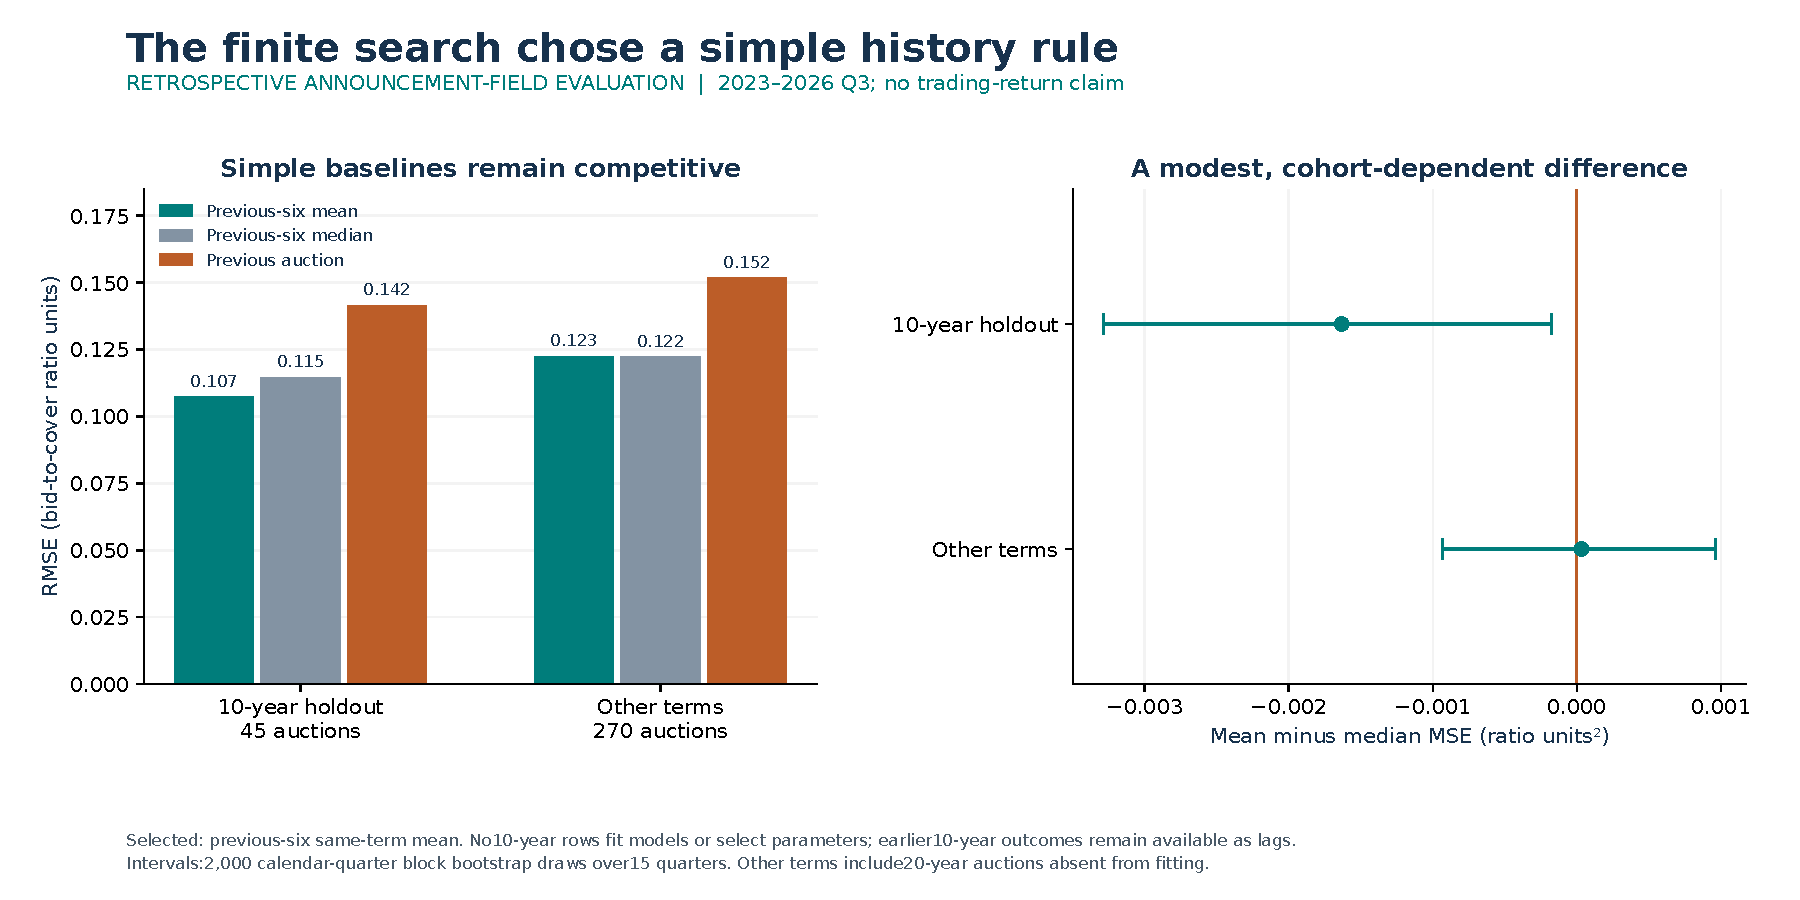
\includegraphics[width=.98\linewidth,height=.86\textheight,keepaspectratio]{images/decision-summary.pdf}
\par\small Figure1. The selected history rule improves modestly on a held-out maturity and is essentially tied elsewhere. Uncertainty uses calendar-quarter blocks.
\clearpage
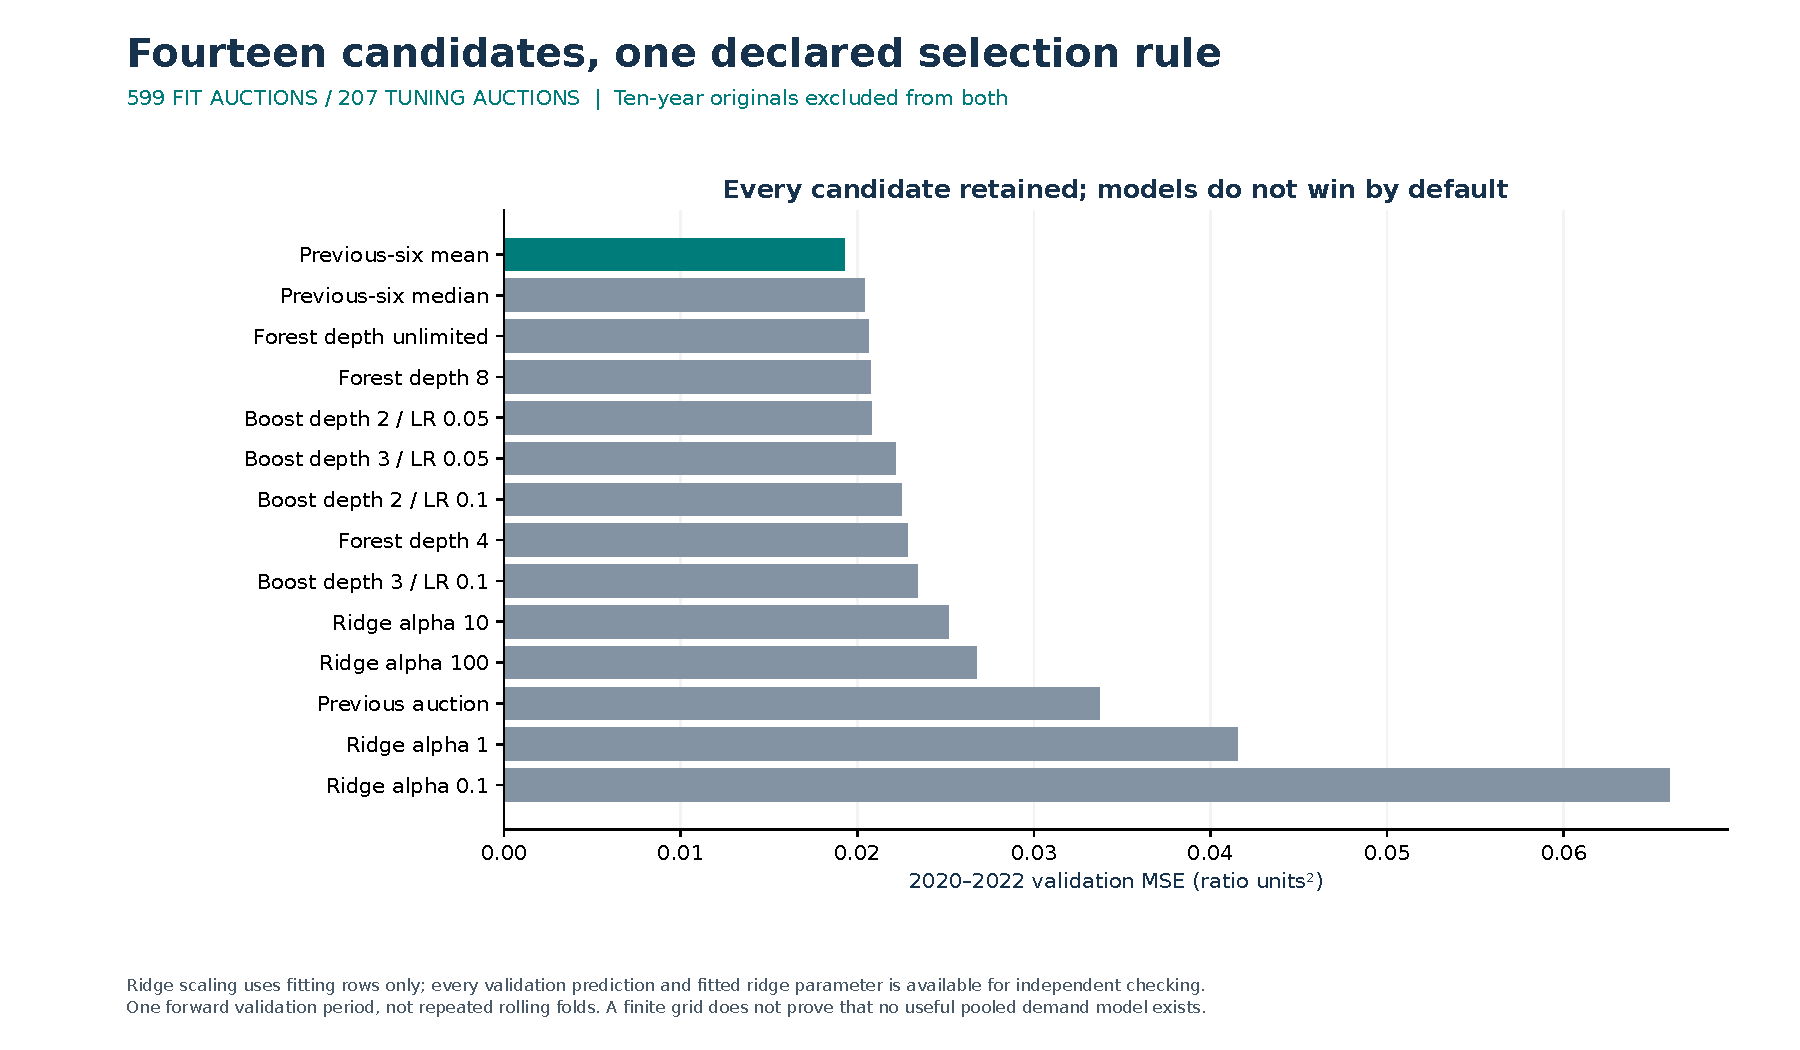
\includegraphics[width=.98\linewidth,height=.86\textheight,keepaspectratio]{images/optimization-evidence.pdf}
\par\small Figure2. All fourteen validation losses are retained. Selection does not privilege a fitted model over a better reference rule.
\clearpage
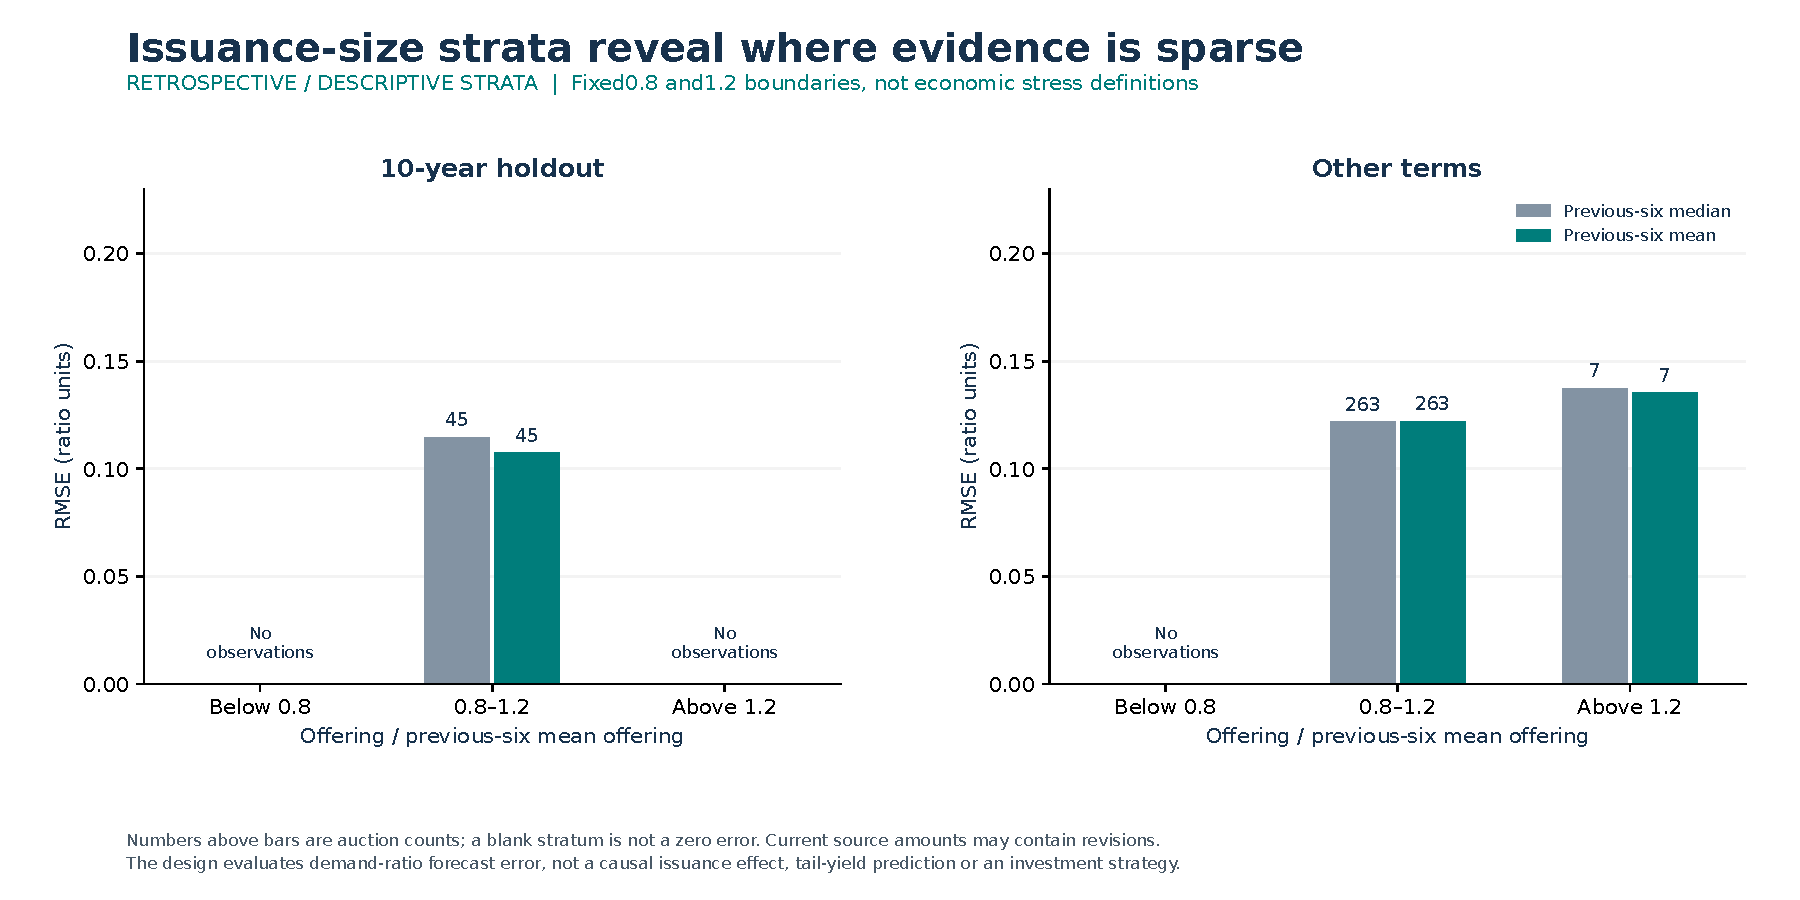
\includegraphics[width=.98\linewidth,height=.86\textheight,keepaspectratio]{images/size-stress.pdf}
\par\small Figure3. Large offering changes are too sparse for a broad stress conclusion. Labels count auctions; missing strata remain explicit.
\end{landscape}\end{document}
